% Use the following line _only_ if you're still using LaTeX 2.09.
%\documentstyle[icml2014,epsf,natbib]{article}
% If you rely on Latex2e packages, like most modern people use this:
\documentclass{article}

% use Times
\usepackage{times}
% For figures
\usepackage{graphicx} % more modern
%\usepackage{epsfig} % less modern
\usepackage{subfigure} 

% For citations
\usepackage{natbib}

% For algorithms
%\usepackage{algorithm}
%\usepackage{algorithmic}
%\usepackage{algorithmicx}

% As of 2011, we use the hyperref package to produce hyperlinks in the
% resulting PDF.  If this breaks your system, please commend out the
% following usepackage line and replace \usepackage{icml2014} with
% \usepackage[nohyperref]{icml2014} above.
\usepackage{hyperref}

% Packages hyperref and algorithmic misbehave sometimes.  We can fix
% this with the following command.
\newcommand{\theHalgorithm}{\arabic{algorithm}}

% Employ the following version of the ``usepackage'' statement for
% submitting the draft version of the paper for review.  This will set
% the note in the first column to ``Under review.  Do not distribute.''
\usepackage{format/icml2014} 
% Employ this version of the ``usepackage'' statement after the paper has
% been accepted, when creating the final version.  This will set the
% note in the first column to ``Proceedings of the...''
%\usepackage[accepted]{icml2014}

\usepackage{times}
\usepackage{hyperref}
\usepackage{url}
\usepackage{color}
\usepackage{preamble}
\definecolor{mydarkblue}{rgb}{0,0.08,0.45}
\hypersetup{ %
    pdftitle={},
    pdfauthor={},
    pdfsubject={},
    pdfkeywords={},
    pdfborder=0 0 0,
    pdfpagemode=UseNone,
    colorlinks=true,
    linkcolor=mydarkblue,
    citecolor=mydarkblue,
    filecolor=mydarkblue,
    urlcolor=mydarkblue,
    pdfview=FitH}
    
    
\usepackage{amsmath, amsfonts, bm, lipsum, capt-of}
\usepackage{natbib, xcolor, wrapfig, booktabs, multirow, caption}
\DeclareCaptionType{copyrightbox}
\usepackage{float}


%\renewcommand{\baselinestretch}{0.99}

\def\ie{i.e.\ }
\def\eg{e.g.\ }
\let\oldemptyset\emptyset
\let\emptyset\varnothing

%\author{
%James Robert Lloyd\\
%University of Cambridge\\
%Department of Engineering\\
%\texttt{jrl44@cam.ac.uk}
%\And
%David Duvenaud\\
%University of Cambridge \\
%Department of Engineering \\
%\texttt{dkd23@cam.ac.uk}
%\And
%Roger Grosse\\
%M.I.T.\\
%Brain and Cognitive Sciences \\
%\texttt{rgrosse@mit.edu}
%\And
%Joshua B. Tenenbaum\\
%M.I.T.\\
%Brain and Cognitive Sciences \\
%\texttt{jbt@mit.edu}
%\And
%Zoubin Ghahramani\\
%University of Cambridge \\
%Department of Engineering \\
%\texttt{zoubin@eng.cam.ac.uk}
%}

\newcommand{\fix}{\marginpar{FIX}}
\newcommand{\new}{\marginpar{NEW}}

\setlength{\marginparwidth}{0.6in}
%%%%%%%%%%%%%%%%%%%%%%%%%%%%%%%%%%%%%%%%%%%%%%%%%%%%%%%%%%
%%%% EDITING HELPER FUNCTIONS  %%%%%%%%%%%%%%%%%%%%%%%%%%%
%%%%%%%%%%%%%%%%%%%%%%%%%%%%%%%%%%%%%%%%%%%%%%%%%%%%%%%%%%

%% NA: needs attention (rough writing whose correctness needs to be verified)
%% TBD: instructions for how to fix a gap ("Describe the propagation by ...")
%% PROBLEM: bug or missing crucial bit 

%% use \fXXX versions of these macros to put additional explanation into a footnote.  
%% The idea is that we don't want to interrupt the flow of the paper or make it 
%% impossible to read because there are a bunch of comments.

%% NA's (and TBDs, those less crucially) should be written so 
%% that they flow with the text.

\definecolor{WowColor}{rgb}{.75,0,.75}
\definecolor{SubtleColor}{rgb}{0,0,.50}

% inline
\newcommand{\NA}[1]{\textcolor{SubtleColor}{ {\tiny \bf ($\star$)} #1}}
\newcommand{\LATER}[1]{\textcolor{SubtleColor}{ {\tiny \bf ($\dagger$)} #1}}
\newcommand{\TBD}[1]{\textcolor{SubtleColor}{ {\tiny \bf (!)} #1}}
\newcommand{\PROBLEM}[1]{\textcolor{WowColor}{ {\bf (!!)} {\bf #1}}}

% as margin notes

\newcounter{margincounter}
\newcommand{\displaycounter}{{\arabic{margincounter}}}
\newcommand{\incdisplaycounter}{{\stepcounter{margincounter}\arabic{margincounter}}}

\newcommand{\fTBD}[1]{\textcolor{SubtleColor}{$\,^{(\incdisplaycounter)}$}\marginpar{\tiny\textcolor{SubtleColor}{ {\tiny $(\displaycounter)$} #1}}}

\newcommand{\fPROBLEM}[1]{\textcolor{WowColor}{$\,^{((\incdisplaycounter))}$}\marginpar{\tiny\textcolor{WowColor}{ {\bf $\mathbf{((\displaycounter))}$} {\bf #1}}}}

\newcommand{\fLATER}[1]{\textcolor{SubtleColor}{$\,^{(\incdisplaycounter\dagger)}$}\marginpar{\tiny\textcolor{SubtleColor}{ {\tiny $(\displaycounter\dagger)$} #1}}}


%% For submission, make all render blank.
%\renewcommand{\LATER}[1]{}
%\renewcommand{\fLATER}[1]{}
%\renewcommand{\TBD}[1]{}
%\renewcommand{\fTBD}[1]{}
%\renewcommand{\PROBLEM}[1]{}
%\renewcommand{\fPROBLEM}[1]{}
%\renewcommand{\NA}[1]{#1}  % Note, NA's pass through!


% The \icmltitle you define below is probably too long as a header.
% Therefore, a short form for the running title is supplied here:
\icmltitlerunning{Automatic construction and natural-language description of nonparametric regression models}

\begin{document} 

\twocolumn[
\icmltitle{Automatic Construction and Natural-language Description \\ of Nonparametric Regression Models}

% It is OKAY to include author information, even for blind
% submissions: the style file will automatically remove it for you
% unless you've provided the [accepted] option to the icml2014
% package.
\icmlauthor{Your Name}{email@yourdomain.edu}
\icmladdress{Your Fantastic Institute,
            314159 Pi St., Palo Alto, CA 94306 USA}
\icmlauthor{Your CoAuthor's Name}{email@coauthordomain.edu}
\icmladdress{Their Fantastic Institute,
            27182 Exp St., Toronto, ON M6H 2T1 CANADA}

% You may provide any keywords that you 
% find helpful for describing your paper; these are used to populate 
% the "keywords" metadata in the PDF but will not be shown in the document
\icmlkeywords{}

\vskip 0.3in
]

%\TBD{ZG: `natural-language summarization' might attract NLP reviewers}
%\TBD{JL: How about `description' - also do we want to say we are doing regression models in the title?}

\begin{abstract} 
%One aim of statistics is to produce accurate and concise descriptions of data.
%Parametric techniques typically produce a concise description of data, but can be inaccurate when there are deviations from the strong assumptions implied by parametric forms.
%In contrast, nonparametric methods are typically capable of providing accurate descriptions of many data sets but at the expense of succinct descriptions.
%To address this apparent antagonism we demonstrate that a recently introduced nonparametric model construction technique allows for the automatic natural-language description of a data set while also constructing an accurate model.
%We also extend the class of models that can be produced by this model construction method to include a wide variety of regression motifs.
We present a nonparametric model construction procedure which also automatically produces natural-language descriptions of the model.
The procedure takes a time-series as input, runs an open-ended model search and then produces a detailed report with figures and english text which decompose and describe the various patterns discovered.
We show how the Gaussian process models being searched over naturally decompose into interpretable structures, which allow simple rule-based descriptions of arbitrarily complex models.
The model search also provides competitive predictive performance.
\end{abstract} 

\allowdisplaybreaks

\section{Introduction}

One of the broad aims of statistics is to produce accurate and concise descriptions of data.
Simple parametric regression models such as linear regression are usually easy to interpret, requiring only a table of regression coefficients and a few other parameters to describe a model.
However, parametric models may often be too simple to accurately describe many data sets.
In contrast, non-parametric regression models are more often able to capture more complex structures but are relatively difficult to summarize, with fitted parameters corresponding only to very high level concepts such as bandwidths or typical lengthscales.
%typically require graphical descriptions of their fit, since any text description would be overly simplistic (\eg `a smooth function') and fitted parameters correspond only to very high level concepts such as bandwidths or typical lengthscales.

Several recently proposed methods search over large classes of structured nonparametric regression models \citep[e.g.][]{diosan2007evolving, bing2010gp, DuvLloGroetal13, kronberger2013evolution}.
In \cite{DuvLloGroetal13} it was noted that these models could be decomposed into sums of diverse components, and that the different components corresponded to interpretable features of the data.
In that work, components discovered by the automatic model search were interpreted post-hoc by the authors.

In this paper, we extend the work of \cite{DuvLloGroetal13} by demonstrating that the compositional structure of the models being searched over allows for the automatic natural-language description of patterns within a data set.
We demonstrate a procedure which, given a dataset, runs an open-ended model search and then produces a detailed report describing the structures discovered by the model. % \ie the interpretable models are automatically interpreted!
%
This paper contains extracts of the natural-language reports automatically generated by our procedure.
The text descriptions within these reports clearly communicate interpretable features of the data, supplemented by appropriate figures.
The supplementary material to this paper includes 13 complete reports generated by our method.

Compared to the work of \cite{DuvLloGroetal13} we also extend and refine the components used in the model-construction process to improve the expressivity and interpretability of the models.
This allows for the procedure to fit and describe many well established modelling motifs including linear regression, Fourier analysis, sparse spectrum \gp{}s \citep{lazaro2010sparse}, changepoints \citep[e.g.][]{garnett2010sequential, FoxDunson:NIPS2012}\fTBD{any suggestions for generic papers? - the Fox paper is quite focused on inference rather than the idea of using changepoints and addition}, heteroscedasiticity, trend-cyclical-irregular \citep[e.g.][]{lind2006basic}\fTBD{Can anyone find a more academic reference?} and additive nonparametric regression \citep[e.g.][]{buja1989linear}\fTBD{Most classical references talk about one smoother per dimension - is MKL a better citation?}.

Finally, we demonstrate that our procedure is comparable or superior to other model construction techniques, in both interpolation and extrapolation tasks.

\section{Background}
\label{sec:gpss}

\subsection{Gaussian process models}

Gaussian processes (\gp{}) \citep{rasmussen38gaussian} can be used to perform Bayesian nonparametric regression.
A \gp{} regression model uses a kernel function, ${\kernel : \mathcal{X}^2 \to \mathbb{R}}$, to define the prior covariance between any two function values, $\outputVar, \outputVar'$ evaluated at two inputs, $\inputVar,\inputVar'$ \ie ${\textrm{Cov}(\outputVar, \outputVar') = \kernel(\inputVar,\inputVar')}$.
The kernel specifies which structures are likely under the \gp{} prior, which in turn determines the generalisation properties of the model.

Different kernels can express a wide variety of structures that one might expect to find in functions.
For example, a \gp{} with a squared-exponential (\kSE) kernel corresponds to a prior on smooth functions.
In contrast, a \gp{} with a periodic (\kPer) kernel corresponds to a prior on periodic functions.
\footnote{The definitions of all kernels are provided in the supplementary material.}

To express richer structures, new kernels can be constructed by taking products of existing ones.
For example, the kernel $\kSE \times \kPer$ puts mass on functions which are locally periodic.
Additive models can also be constructed by taking sums of kernels.
For example, a \gp{} with kernel $\kSE + \kLin$ corresponds to a prior on smooth functions with a linear trend.
A more detailed discussion with examples can be found in \cite{DuvLloGroetal13} and at \url{http://mlg.eng.cam.ac.uk/duvenaud/cookbook/}.

\subsection{Gaussian Process Structure Search}

The Gaussian process structure search (GPSS)\fTBD{RG: More specific name?} procedure \citep{DuvLloGroetal13} searches over sums and products of a set of simple base kernels to produce an appropriate model for a data set.
The properties of \gp{}s and the structured nature of the kernels produced allows for the models to be decomposed into a sum of interpretable components.

Since the search operates over an open-ended language of kernel structres, it can construct novel nonparametric regression models.
For example, when applied to airline passenger data (section~\ref{sec:airline}), the resulting kernel contained a component of the form $\kSE \times \kPer \times \kLin$, which can be described as ``locally periodic, with linearly growing amplitude''.
In \citep{DuvLloGroetal13}, the authors plotted these discovered components, and described each one by hand.

In this paper we show that one can automatically generate natural-language descriptions of \gp{} models in this open-ended class.
Combined with relevant plots of components of the posterior, our system automatically generates detailed reports discussing the varied structures present in a dataset.
This system represents the beginnings of an ``automatic statistician'', which has the potential to aid in exploratory analysis of data.

%\subsection{Paper Outline}
%
%Section \ref{sec:improvements} reviews the language of models searched over by the GPSS procedure, introducing extensions and refinements.
%We describe how any model in this class can be automatically described in natural language in section~\ref{sec:description}.
%We discuss excerpts of the reports produced by GPSS in section~\ref{sec:examples}.
%Section \ref{sec:numerical} compares the predictive power of GPSS against other model construction techniques.
%As supplementary material we have included reports produced by our method on all of the 13 datasets used in section \ref{sec:numerical}.

\section{A language of regression models}
\label{sec:improvements}

The work of \cite{DuvLloGroetal13} constructed a language of regression models by mutiplying and adding four base kernels.
These four base kernels were $\kSE$ (smooth), $\kLin$ (linear), $\kPer$ (periodic), and $\kRQ$ (multi-scale smoothness).
By combining these kernels, many structures can be expressed, such as periodic functions with long-term trends, or short-term deviations with linearly increasing amplitude through time.

In this section we extend the language to include a greater variety of regression motifs.
We also modify the base kernels to allow more succinct descriptions of the models produced.

%to improve\fTBD{RG: Do we have direct comparisons JL: No - but we can demonstrate negative properties of previous of previous work if desired} the interpretability of the models produced by GPSS where we are guided by the principle that \emph{a model is interpretable if it can automatically be described in natural language}\fTBD{RG: Controversial}.

\subsection{Changepoints}

The original GPSS language could not capture the non-linear non-stationarity exhibited in a solar irradiance data set (section~\ref{sec:solar}).
To capture this type of phenomenon, we introduce changepoints into the modeling language.

Hard changepoints have been considered by \citep[e.g.][]{garnett2010sequential, FoxDunson:NIPS2012}.
We construct smooth changepoints by multiplying by sigmoidal functions.
\fTBD{DD: Let's add a small figure here to show what changepoints can do.}
Suppose that $f_1(x) \dist \gp{}(0, \kernel_1)$ and $f_2(x) \dist \gp{}(0, \kernel_2)$ and define
\begin{align}
f(x) = \sigma(x)f_1(x) + (1-\sigma(x)) f_2(x)
\end{align}
where $\sigma(x)$ is a sigmoid function varying between 0 and 1, so that $f$ transitions between functions $f_1$ and $f_2$.
Then $f(x) \dist \gp{}(0,\kernel)$ where
\begin{align}
\kernel(x,x') = \qquad \qquad \sigma(x) & k_1(x,x')\sigma(x') \nonumber \\ + (1-\sigma(x)) & k_2(x,x')(1-\sigma(x'))
\label{eq:cp}
\end{align}
%(see section~\ref{sec:description} for the properties to prove this identity).
%
We represent this kernel with the changepoint operator $\kCP(\kernel_1, \kernel_2)$.
We also introduce a change window operator, $\kCW(\cdot,\cdot)$, which uses a product of two sigmoids to produce a smooth `hat-shaped' modulation of a function.

\paragraph{Heteroscedasticity}

To more flexibly model different types of noise, we introduce the white noise kernel, $\kWN$, as a base kernel.  Combined with linear kernels and changepoints, this addition allows models with noise levels which vary over time.
%When multiplied by linear kernels and changepoints, this can express polynomially varying standard deviation as well as switching between different noise regimes.
%The original GPSS procedure always assumed homoscedastic noise.

\paragraph{A separate constant kernel}
% included in typical definitions of $\kLin$ and $\kPer$ kernels.
The $\kLin$ and $\kPer$ are typically parameterized with an implicit constant added.  By introducing a constant kernel $\kC$ we can remove this constant component in order to more clearly decompose the different types of structure present.
%The new form of linear kernel is necessary for the modular construction of descriptions of kernels (see section [blank]).

This new form of periodic kernel\footnotemark~includes the cosine kernel as a limiting form.
It was recently demonstrated \citep{WilAda13} that any stationary kernel can be arbitrarily well approximated by kernels of the form $\sum \kSE \times \cos$ by appealing to Bochner's theorem \citep{bochner1959lectures}.
By using this new periodic kernel our language of kernels also attains this completeness property.
More details are in the supplementary material.

\footnotetext{This kernel is now included in the GPML toolbox (\url{ www.gaussianprocess.org/gpml/code/}) as \texttt{covPeriodicNoDC}}

\paragraph{Removal of $\kRQ$}
The $\kRQ$ kernel is equivalent to a mixture of $\kSE$ covariance functions with different length-scales.
In preliminary testing we observed that this allowed the kernel to simultaneously model aspects of the data that might be considered signal and noise.
We therefore removed this kernel to improve the interpretability of the models produced.

\subsection{A broad language of statistical models}

With these additions to the modelling language, we can express a wide variety of regression motifs, shown in table~\ref{table:motifs}.

\begin{table}[ht]
\centering
\begin{tabular}{l|l}
Motif & Example syntax \\
\midrule
Linear regression & $\kC + \kLin$ \\
Fourier analysis* & $\kC + \sum \cos$ \\
Sparse spectrum* \gp{}s & $\sum \cos$ \\
Spectral kernels* & $\sum \SE \times \cos$ \\
Changepoints* & \eg $\kCP(\kSE, \kSE)$ \\
Kernel smoothing & $\kSE$ \\
Heteroscedasticity* & \eg $\kSE + \kLin \times \kWN$ \\
Trend cyclical irregular & $\sum \kSE + \sum \kPer$ \\
Additive nonparametric & $\sum \kSE$ \\
\end{tabular}
\caption{
Syntax of common regression motifs expressible in our language. * denotes a motif not present in the original grammar.
}
\label{table:motifs}
\end{table}

%In section~\ref{sec:example_description} we demonstrate the natural-language descriptions of some of these kernel forms.

\section{Automatic natural-language description of regression models}
\label{sec:description}
%\fTBD{RG: Does the algorithm clarify anything?}
%\fTBD{RG, JBT: Section unclear} 

In this section we describe how the properties of \gp{} models allow one to reduce the task of describing the model produced by an arbitrary kernel expression into simple subproblems.
%The text follows the flow of algorithm~\ref{alg:description}.

\subsection{Modular description of arbitrary kernel expressions}

\subsubsection{Overview}

The automatic description procedure begins by distributing a kernel expression into a sum of products and then applying simplification operations.
A sum of kernels corresponds to a sum of functions which allows each product of kernels to be described separately.
Changepoints and linear kernels have a special form allowing them to be described independently of other kernels in a product.
After the simplification operations there are relatively few combinations of the other kernels so their descriptions are templated based on their parameter values.
The procedure is outlined in algorithm~\ref{alg:description}.

%Generating descriptions for any product of kernels is possible because, conveniently, multiplying any kernel by a base kernel modifies the properties of the resulting model in consistent ways. Loosely speaking, each kernel corresponds to an adjective in the model description.

%For example, multiplying any kernel by \kPer makes the resulting model periodic.
%The exact effect that each component of the product has depends on the hyperparameters of each kernel.

%Each of these separate description tasks is now small enough that sentences can be templated based on parameter values and basic properties of the posterior.

\begin{algorithm}[tb]
   \caption{Natural-language Description of Model}
   \label{alg:description}
\begin{algorithmic}
   \STATE {\bfseries Input:} kernel expression $e$
   %\STATE $e = {ChangePointsToSumsAndProducts}(e)$
   \STATE $e = {\textnormal{ \sc SumOfProductsForm}}(e)$
   \STATE $e = {\textnormal{ \sc Simplify}}(e)$
   \FOR{$k$ in {\sc SummandsOf}$(e)$}
   \STATE {\textnormal{ \sc DescribeStationaryComponents}} $(k)$
   \STATE {\textnormal{ \sc DescribeLinearComponents}} $(k)$
   \STATE {\textnormal{ \sc DescribeChangepointComponents}} $(k)$
   %\STATE \COMMENT{Individual summands can be described separately}
    % \REPEAT
    % \UNTIL $k$ is unchanged
       %\FOR{$m$ in {\sc ProductsOf}$(k)$}
            %\STATE {\textnormal{ \sc Describe}} $(m)$
     %\STATE $DescribeChangePointComponents(k)$
     %\STATE $DescribeStationaryComponents(k)$
     %\ENDFOR
   \ENDFOR
\end{algorithmic}
\end{algorithm}

\subsubsection{Sum of products form}

Pointwise multiplication is distributive over addition for functions so we can distribute kernel multiplication over addition \eg $\kSE \times (\kC + \kLin) = \kSE \times \kC + \kSE \times \kLin$.

Changepoints can also be represented as a sum of products; from equation \eqref{eq:cp} we can write
\begin{equation}
\kCP(k_1, k_2) = \bar\Sigma\times k_1 + \Sigma \times k_2
\end{equation}
where $\Sigma = \sigma(x)\sigma(x')$ and $\bar\Sigma = (1-\sigma(x))(1-\sigma(x'))$.
Changewindows can be represented similarly.

After converting changepoints and changewindows into the form above and distributing multiplication over addition any kernel expression can be converted into a sum of products of the form
\begin{equation}
\prod_i k_i\prod_j\kLin_j\prod_m\Sigma_m
\label{eq:sop}
\end{equation}
where the $k_i$ are base kernels excluding $\kLin$ and the $\Sigma_m$ are products of sigmoids.

\subsubsection{Sums of kernels are sums of functions}

If $f_1(x) \dist \gp{}(0, \kernel_1)$ and $f_2(x) \dist \gp{}(0, \kernel_2)$ then $f_1(x) + f_2(x) \dist \gp{}(0, \kernel_1 + \kernel_2)$.
Therefore, each product of kernels corresponds to an independent additive function in the model and can be described separately.

\subsubsection{Simplification}

Ignoring the specific parameters of kernels, $\kSE$ is multiplicatively idempotent \ie $\kSE \times \kSE = \kSE$ (simply, the product of two $\kSE$ kernels is another $\kSE$ kernel but with different parameters).
Similarly, $\kWN$ and $\kC$ are additively idempotent.

For stationary kernels, $\kWN$ behaves like a multiplicative zero \eg $\kWN \times \kSE = \kWN \times \kPer =  \kWN$.
The constant kernel $\kC$ behaves like a multiplicative identity \eg $\kC \times \kLin = \kLin$.

\subsubsection{Kernel description templates}

After applying all simplifications to a kernel expression in sum of products form the product of base kernels (excluding $\kLin$) will have of the following forms: $\kWN, \kC, \kSE, \kPer^n, \kSE\times\kPer^n$ where $n\in\mathbb{N}$.

The models produced by the base kernels are well understood so appropriate templates for their descriptions based on parameter values can be constructed from standard reference books \citep[e.g.][]{rasmussen38gaussian}.

A description for $\kPer^n$ with ${n>1}$ can be constructed as follows.
Suppose that ${f_1(x) \dist \gp{}(0, \kernel_1)}$ and ${f_2(x) \dist \gp{}(0, \kernel_2)}$.
Then
\begin{equation}
{\textrm{Cov} \left[f_1(x)f_2(x), f_1(x')f_2(x') \right] = k_1(x,x')k_2(x,x')}.
\end{equation}
Therefore $\kPer \times \kPer$ defines a prior on functions whose covariance is the same as the product of independent periodic functions.
This description naturally extends to ${n>2}$.
However, note that a product of periodic functions drawn from \gp{} priors will not be distributed according to a \gp{}.

A description for $\kSE\times\kPer$ can be constructed as follows.
If the input space is restricted to a grid with spacing equal to the period of the periodic kernel, then $\kSE \times \kPer = \kSE$.
That is, the functional form of the periodicity varies like $\kSE$, giving rise to local periodicity.
This argument extends to $\kSE\times\kPer^n$ again producing locally periodic functions.

\subsubsection{Linear kernels}

$\kLin$ has the form $k(x,x') = a(x)a(x')$.
This can be used as follows: suppose that $f(x) \dist \gp{}(0, \kernel)$ and $a : \mathcal{X} \to \mathcal{Y}$ is a deterministic function.
Then $a(x)f(x) \dist \gp{}\left(0, a(x) k(x, x') a(x') \right)$.
Therefore multiplying a kernel, $\kernel$, by the linear kernel is equivalent to multiplying $f(x) \sim \gp{}(0, k)$ by a linear function.

This allows us to describe any linear kernels separately.
For example, multiplying by a linear kernel means that the amplitude of the function grows linearly away from a central point.
Multiplication by two linear kernels results in quadratic growth, etc.

\subsubsection{Changepoints}

The $\Sigma_m$ in the sum of products form shown in equation~\eqref{eq:sop} represent products of sigmoids which also have the form $a(x)a(x')$.
For the purposes of description we assume that the sigmoids are step functions (the parameters of the sigmoids are restricted to make the sigmoids step and therefore this approximation is not severe).

These step functions can be represented as intervals (\ie where their value is 1), and their product is equivalent to taking the intersection of intervals.
Computing the intersection is trivial and descriptions can be templated as `this function applies from [start] until [end]'.

\subsection{Worked example}

Suppose we start with a kernel of the form
\begin{align*}
\kSE \times (\kWN \times \kLin + \kCP(\kC, \kPer)).
\end{align*}
This is converted to sum of products form
\begin{align*}
\kSE \times \kWN \times \kLin + \bar\Sigma\times\kSE \times \kC + \Sigma\times\kSE \times \kPer.
\end{align*}
which can be simplified to
\begin{align*}
\kWN \times \kLin + \bar\Sigma\times\kSE + \Sigma\times\kSE \times \kPer.
\end{align*}
Note that this can equivalently written as
\begin{align*}
\kWN \times \kLin + \kCP(\kSE, \emptyset) + \kCP(\emptyset, \kSE \times \kPer)
\end{align*}
where $\emptyset$ represents the zero function.
We use this notation in section~\ref{sec:solar}.

To descibe the first component, the template for $\kWN$, `uncorrelated noise', is concatenated with a template (chosen based on parameter values) for $\kLin$, `with linearly increasing standard deviation'.

The second component could be described as `A smooth function with a lengthscale of [lengthscale]', corresponding to the $\kSE$, 'which applies until [changepoint]', which corresponds to the $\bar\Sigma$.

Finally, the third component could be described as `A locally periodic function with a period of [period] which applies from [changepoint]'.

\subsection{Breaks from modularity and other corner cases}

We use a separate template for $\kLin$ when there are no stationary kernels present \eg `a linear/quadratic/cubic function'.
When both $\kPer$ and $\kLin$ are present in a product we change the template for $\kLin^n$ from discussing `varying standard deviation' to `varying amplitude'.
These separate cases are not necessary but make the generated text more natural.

We also use different templates to produce short summaries and detailed descriptions of kernels.

\subsection{Ordering additive components}

The reports generated by GPSS attempt to present the most interesting or important features of a data set first.
As a heuristic, we order components by adding the component which most reduces the 10-fold mean absolute error (using a contiguous block design) when added to the model.
This procedure is iterated to produce a complete ordering.

\subsection{When is a description of a model useful as a description of data?}

GPSS produces models, $M$, of the form $f = \sum_i f_i$ where $f_i \dist \gp{}(0, \kernel_i)$.
The form of $M$ is chosen to be that which best explains observations of $f$, denoted by $D$, as measured by approximate marginal likelihood.

In the reports generated by GPSS we show plots of the posterior $p(f_i^*\given M,D)$ but the natural-language descriptions are of typical elements of the prior $p(f_i^*\given M)$ given the fitted model \ie they are descriptions of the model rather than descriptions of the data.

Despite fitting the model to the data by maximising the marginal likelihood $p(D\given M)$ the selected model may be a poor description of the data if the data contains features not easily expressed by the language of models defined by GPSS.
To test for when this is the case we have begun experimenting with posterior predictive checks to assess the models produced by GPSS following the techniques of \cite{Gelman1996} (see reports in the supplementary material).
In fact, the posterior predictive checks take the form of comparing the expectation of statistics under the prior and posterior of each component \ie they are testing whether or not typical elements of the posterior $p(f_i^*\given M,D)$ are typical elements of $p(f_i^*\given M)$.

However, model checking for Gaussian processes, even those with simple kernels, is under-researched so we leave their description and more detailed analysis for future work.

%The kernel learned for solar was:
%\begin{align*}
%\kWN + \kC + \kCW(\kSE + \kSE + \kSE \times \kLin  + \kSE \times \kLin + \kSE \times \kPer, \kC)
%\end{align*}
%which is already in sum of products form except for the changewindow.
%Distributing the changewindow results in the following additive components: $\kC$, $\kCW(\kC)$, $\kCW(\kSE)$, $\kCW(\kSE \times \kPer)$, $\kCW(\kSE)$, $\kWN$, $\kCW(\kSE \times \kLin)$, and $\kCW(\kSE \times \kLin)$

%The first component, $\kC$ is the constant kernel - its description can be looked up.

%The second component, $\kCW(\kC)$, is the constant base kernel within a changewindow operator.
%By inspecting the parameters of the change window, it can be deduced that this component is zero except in the region from 1644 to 1713\fTBD{It currently does not comment on the speed/slope of the transition} which can be translated using an appropriate template \eg `this function applies from 1644 until 1713'.
%The constant base kernel is then described separately by looking up its description.

%The third component, $\kCW(\kSE)$, is similar to the second, but the $\kSE$ requires more description than $\kC$.
%The lengthscale of the $\kSE$ is compared to the range of the input dimension of the data to determine an appropriate template to use (\ie is the function very smooth, smooth or quickly varying?).
%For this component, the lengthscale is moderate so the function is described as smooth.

%The changewindow aspect of the fourth component, $\kCW(\kSE \times \kPer)$, is dealt with in the same manner as the above.
%There are different templates for the $\kSE \times \kPer$ kernel expression which are selected based on the parameter values of the kernels in comparison to the dimensions of the dataset.

%The seventh component, $\kCW(\kSE \times \kLin)$, is also translated in a modular fashion.
%The changewindow is translated as before from a template 'This component applies until 1643 and from 1716 onwards'.
%The linear kernel is translated separately, using an appropriate template based on parameter values resulting in `The marginal standard deviation of the function increases linearly away from 1701'.
%The $\kSE$ is translated spearately from a template `This component is a rapidly varying but smooth function with a typical lengthscale of 2.2 months'.
%The full description is actually these sentences in reverse order.

%\subsection{Describing products of kernels}

%The extended GPSS language produces sentences composed of 5 base kernels (section~\ref{sec:notation}) and the arbitrary application of addition, multiplication, change point and change window operators. 

%\paragraph{Changepoints}

%We use equation \eqref{eq:cp} to represent changepoints (and similarly change windows) using sums, products, base kernels and sigmoid functions.

%\paragraph{Distributivity}

%Pointwise multiplication is distributive over addition for functions so we can convert any kernel expression into a sum of products.

%\paragraph{Changepoints and changewindows}

%Representing changepoints/windows as sigmoid functions as shown in equation~\eqref{eq:cp} also results in kernels of the form $a(x)k(x,x')a(x')$ where $a(x)$ is a sigmoid (changepoint) or product of sigmoids (changewindow).
%Therefore the application of changepoint/window operators can be described separately as multiplication of functions by sigmoids.
%When the sigmoids transition between 0 and 1 sharply the effect is particularly trivial to express in natural-language \eg ``this component applies from 1700 to 1800''.

%We now only need to describe the base kernels and products of the form $\kSE \times \prod \kPer$.

%\paragraph{Base kernels}

%The priors induced by the base kernels are well understood, with simple descriptions of typical functions.

%\vspace{-0.5\baselineskip}
%\begin{table}[ht]
%\centering
%\begin{tabular}{c|c}
%Kernel & Function description \\
%\midrule
%$\kWN$ & White noise \\
%$\kC$ & Constant \\
%$\kLin$ & Linear \\
%$\kSE$ & Smooth \\
%$\kPer$ & Periodic \\
%\end{tabular}
%\label{table:base-kernels}
%\end{table}
%\vspace{-\baselineskip}

%\paragraph{Products of multiple periodic kernels}

%Suppose that ${f_1(x) \dist \gp{}(0, \kernel_1)}$ and ${f_2(x) \dist \gp{}(0, \kernel_2)}$.
%Then
%\begin{equation}
%{\textrm{Cov} \left[f_1(x)f_2(x), f_1(x')f_2(x') \right] = k_1(x,x')k_2(x,x')}.
%\end{equation}
%Therefore $\kPer \times \kPer$ defines a prior on functions whose covariance is the same as the product of independent periodic functions.  However, note that a product of periodic functions drawn from \gp{} priors will not be distributed according to a \gp{}.

%\paragraph{Description is modular}

%Linear kernels have special form and can be translated separately.
%Changepoints, when split into additive components also have this form and can therefore also be translated separately.

%\paragraph{Description of changepoints}

%A combination of changepoints and changewindows specifies a collection of intervals to which a function applies.
%These intervals are easy to calculate from parameter values and we only need templates for open at the left, closed, open at the right intervals  and appropriate connectives.

%\paragraph{Description of linear kernels}

%Products of linear kernels are easily described as `linear', `quadratic', `cubic', etc.

%\subsection{Description of compound kernels}

%After simplification, there are only a small number of kernels we need to create templates for: $\kWN$, $\kC$, $\kSE$, $\prod \kPer$, and $\kSE \times \prod \kPer$.

%We include a few variants of the templates depending on kernel parameters and simple statistics of the posterior (\eg very smooth functions, monotonicity).

%The base kernels have well defined descriptions in the literature.
%The product of periodics has the same covariance as a product of functions - allowing for a simple template description.
%Multiplication by $\kSE$ has a localising effect which again allows for easy templating of a description.

%In principle we could create templates for $\SE \times k$ and $\Per \times k$ for arbitrary $k$ since these have consistent `localising' and `making periodic' effects respectively.
%This isn't so important at the moment, but if the base kernels expand we may need to exploit this additional modularity.

%\subsection{In practice}

%Special cases are included to improve readability.
%For example, a product of linear kernels has its own template.
%Also, `periodic with linearly increasing amplitude' is not an entirely modular construction.

\section{Natural-language description of time series}
\label{sec:examples}
We demonstrate the ability of our procedure to describe a variety of patterns on two time series (full automatically produced reports for 13 data sets are provided as supplementary material).
The automatic natural-language descriptions objectively demonstrate that the models can be interpreted.
However, it is difficult to quantify the quality of a verbal description so we also provide numerical evidence in support of our procedure in section~\ref{sec:numerical}.

%Our report generation procedure takes as its starting point a dataset and a composite kernel, which together define a joint posterior probability distribution over a sum of functions.
%The procedure summarizes properties of this complex distribution to the user through a comprehensive report.
%
%These reports are designed to be intelligible to non-experts, illustrating the assumptions made by the model, describing the model's posterior distribution, and most importantly, enabling model-checking.
%\subsection{Design goals}
%
%\begin{itemize}
%\item {\bf Intelligibility}
%The procedure was designed to produce reports intelligible to non-experts.  
%
%\item {\bf Illustrate Model Assumptions}
%One of the main design criteria when designing our procedure was to make clear what assumptions the model is making, and what these assumptions imply in terms of extrapolation.  Even when simple Gaussian process models are used, it is often unclear what structure was captured by the model and what was not.
%
%\item {\bf Illustrate Posterior Uncertainty}
%One of the selling points of Bayesian modeling over point estimates is that they produce a rich posterior distribution over possible explanations of the data.  However, this posterior distribution is often quite a complex object, and is usually difficult to summarize.
%
%\item {\bf Enable Model-checking}
%One of the most important reasons to examine a model is to discover flawed assumptions, or structure not captured by the model.  Simply examining residuals, cross-validation or marginal likelihood scores is often not sufficient to notice when the model is failing to capture.
%\end{itemize}
%
%\subsection{Report structure}

%These reports have three sections: an executive summary, a detailed discussion of each component, and a section discussing how the model extrapolates beyond the range of the data.

%\vspace{-0.05in}

\subsection{Summarizing 400 Years of Solar Activity}
\label{sec:solar}

\begin{figure}[h]
\centering
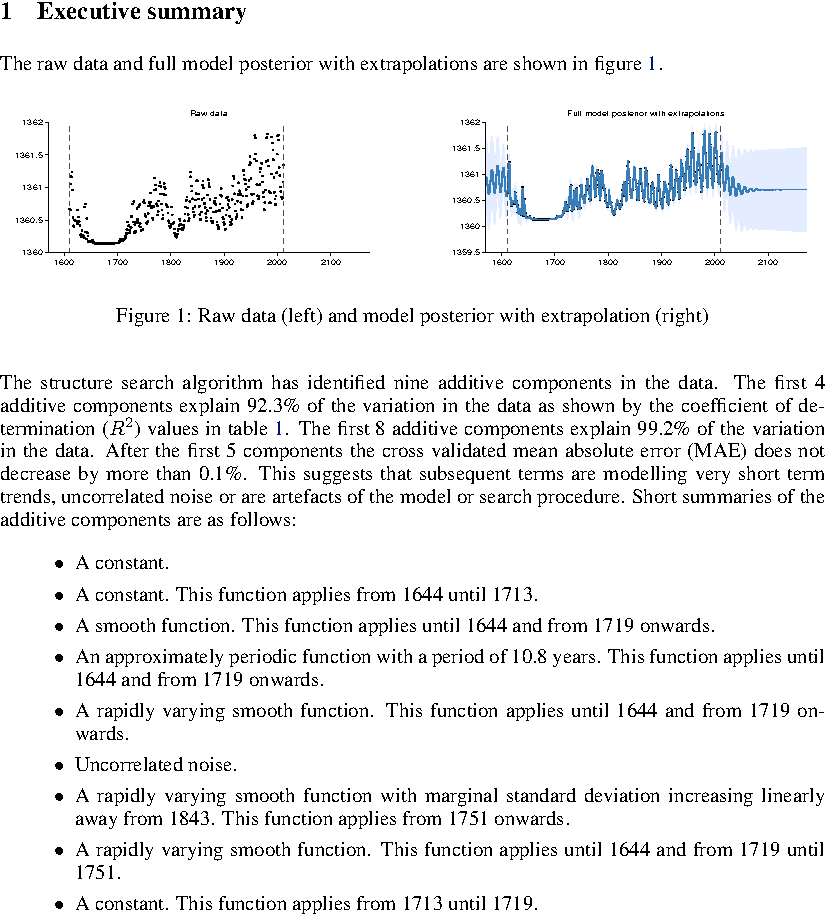
\includegraphics[trim=0cm 11.0cm 9cm 1.7cm, clip, width=0.98\columnwidth]{solarpages/02-solar-seperate-pages-2}
\caption{
Solar irradiance data.}
\label{fig:solar}
\end{figure}

We show excerpts from the report automatically generated on annual solar irradiation data from 1610 to 2011 (figure~\ref{fig:solar}).
This time series has two pertinent features: a roughly 11-year cycle of solar activity, and a period lasting from 1645 to 1715 with much smaller variance than the rest of the dataset.  This flat region corresponds to the Maunder minimum, a period in which sunspots were extremely rare \citep{lean1995reconstruction}.
The GPSS search procedure and automatic description clearly identify these two features, as discussed below.

\paragraph{Summary of main features}

The kernels corresponding to the first four components are as follows:
\vspace{-0.5\baselineskip}
\begin{itemize}
  \itemsep0em
  \item $\kC$
  \item $\kCW(\emptyset,\kC)$
  \item $\kCW(\kSE,\emptyset)$
  \item $\kCW(\kSE \times \kPer,\emptyset).$
\end{itemize}
\vspace{-\baselineskip}

\begin{figure}[h]
\centering
\fbox{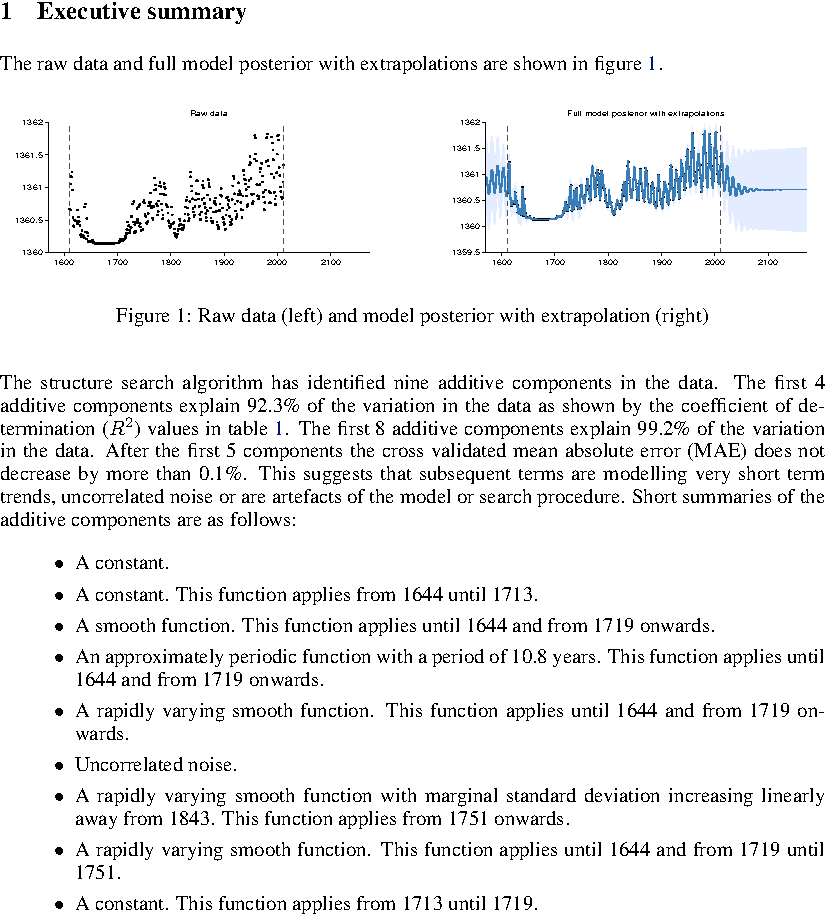
\includegraphics[trim=0cm 3.4cm 0cm 6.3cm, clip, width=0.98\columnwidth]{solarpages/02-solar-seperate-pages-2}}
\caption{
An example of an automatically-generated summary of a dataset.  The dataset is decomposed into diverse structures with simple descriptions.}
\label{fig:exec}
\end{figure}
Figure \ref{fig:exec} shows the natural-language summaries of these components produced by GPSS.
%The short descriptions demonstrate how the kernel is split into univariate enveloping functions (from the change windows) and stationary kernels.
%
%
%The model uses 9 additive components to explain the data, and reports that the first 4 components explain more than 90\% of the variance in the data.
%This might seem incongruous with the observation that there are two main features of the data, but if we examine the first four components, we see that the first component is describing the mean of the dataset, the second is the Maunder minimum, the third describes the long-term trend, and the fourth describes the 11-year periodicity.
Just from the short summaries of the additive components we can see that the model has identified the Maunder minimum (second component) and 11-year solar cycle (fourth component).
We now discuss these components in greater detail.
%This might seem incongruous with the observation that there are two main features of the data, but if we examine the first four components, we see that the first component is describing the mean of the dataset, the second is the Maunder minimum, the third describes the long-term trend, and the fourth describes the 11-year periodicity.

%\subsubsection{Signal versus Noise}
%
%One design challenge we encountered was seperating the recovered structure into signal and noise.  Originally, the model always included a term corresponding to \iid{} additive Gaussian noise.  However, in practice, the distinction between signal and noise is unclear for two reasons.  First, a component which varies arbitrarily quickly in time can be indistinguishable from noise.  Second, the variance of the noise may change over time (called heteroscedasticity), and this sort of pattern may be considered part of the signal.
%Because of the blurry distinction between signal and noise, we include a table which summarizes the relative contribution of each component in terms of held-out predictive power.%  To do this, we order the components in terms of how much each one improves predictive performance in a 10-fold cross-validation procedure.  The intuition for this metric is that noise-like components do not contribute much to the extrapolation performance of the model, but that signal-like components do.
%
%
%\begin{figure}
%\centering
%\fbox{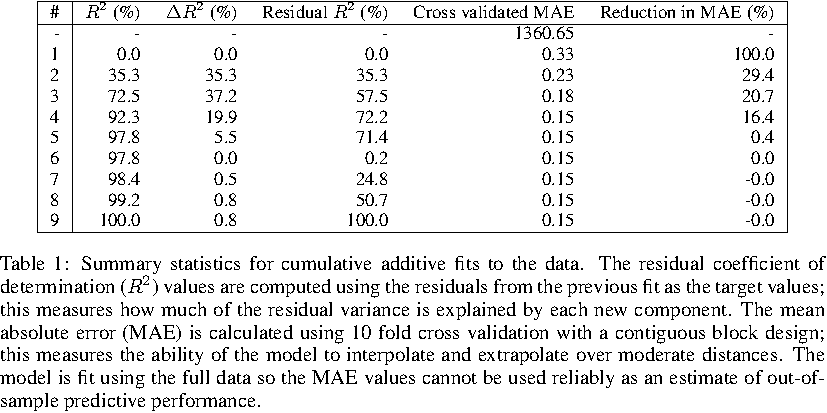
\includegraphics[width=0.98\columnwidth]{solarpages/02-solar-seperate-pages-3}}
%\caption{A table summarizing the relative contribution of the 9 different components of the model in terms of predictive performance.}
%\label{fig:table}
%\end{figure}
%
%Figure \ref{fig:table} show an example of this table on the solar dataset.

%Because the user may be interested in local or noisy components, we report all components to the user.  
%An interactive version of our procedure could allow users to specify which components are of interest, and group the remaining components into a single noise component.

%\paragraph{Decomposition plots}

%The second section of each report contains a detailed discussion of each component.
%Every component is plotted, and properties of the covariance structure are described.
%Some components are not meaningful when plotted on their own, so we also include plots of the cumulative sum of components.
%\paragraph{Automatic Plotting}
%The posterior of the individual component and sum of all components so far is visualised by plots of the posterior mean and variance.
%First, the posterior mean and variance of each component is plotted on its own.
%Second, the posterior mean and variance of all components shown so far is plotted against the data.
%This progression of plots 
%By contrasting each of these plots with plots of earlier components, we can see 
%shows qualitatively how each component contributes to an overall explanation of the data.

%A second paragraph explains the improvement in predictive performance gained by including this component in the model. This is the same informatino as included in the executive summary.

\paragraph{Maunder minimum}

Figure \ref{fig:maunder} shows that GPSS has captured the unusual period of decreased solar activity from about 1645 to 1715 and is able to report this in natural language.

\begin{figure}[ht]
\centering
\fbox{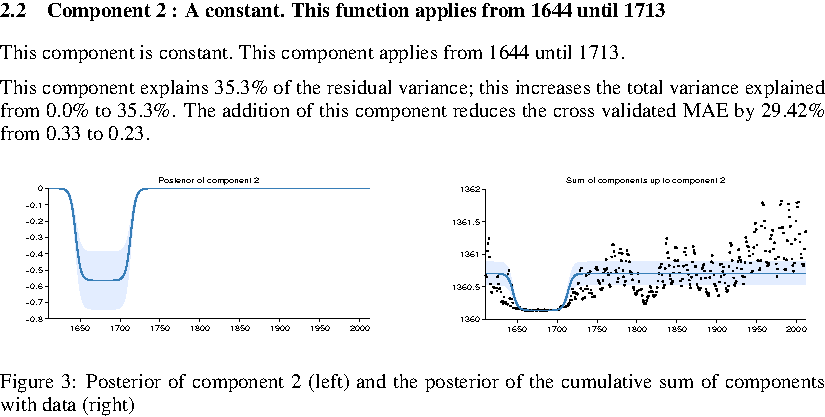
\includegraphics[trim=0cm 0cm 0cm 0.7cm, clip, width=0.98\columnwidth]{solarpages/02-solar-seperate-pages-5}}
\caption{Discovering the Maunder minimum.}
\label{fig:maunder}
\end{figure}

\paragraph{Long term trend}

Having isolated the Maunder minimum, the model captures the long term trend of the rest of the data, shown in figure~\ref{fig:smooth}.

\begin{figure}[h!]
\centering
\fbox{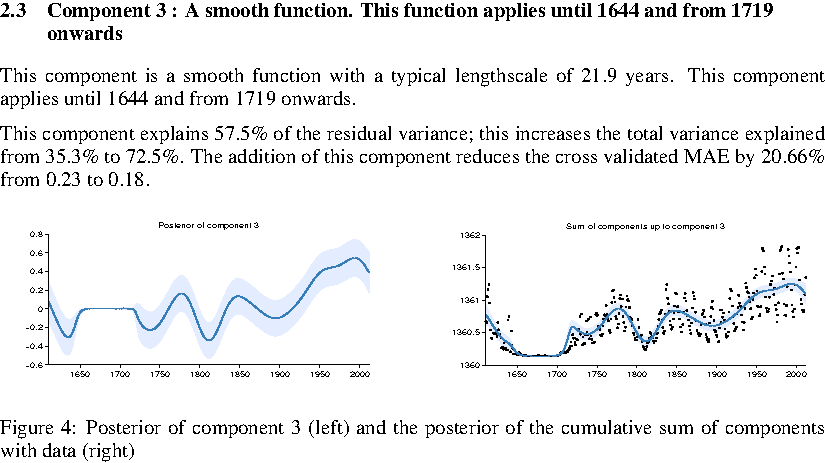
\includegraphics[width=0.98\columnwidth]{solarpages/02-solar-seperate-pages-6}}
\caption{Characterizing the medium-term smoothness of solar activity levels.  By allowing other components to explain the periodicity, noise, and the Maunder minimum, we can isolate the part of the signal best explained by a slowly-varying trend.}
\label{fig:smooth}
\end{figure}

% is a good example of a meaningful component discovered by GPSS, whose meaning would be unclear without an individual plot.  


%In the history of solar activity, the Maunder minimum is a good example of a local change in covariance.  Specifically, 
%The changepoint kernels used by GPSS encode changes in covariance structure.
%For example, from about 1645 to 1715, solar activity decreased.
%, and very few sunspots were observed, a period called the Maunder Minimum \citep{lean1995reconstruction}.
%This feature was captured by the model by multiplying a constant kernel by two changepoint kernels.

\paragraph{Solar cycles}

Figure \ref{fig:periodic} shows that GPSS has isolated the approximately 11 year solar cycle.
By examining the parameters of the kernels comprising this component the description identifies that the shape of the periodicity is near sinusoidal \TBD{(it does in the latest version - update me)} and also quantifies how quickly the exact shape of the sinusoid changes.

%with a pair of changepoint kernels.%shows exactly which sort of structure was recovered by this component.
%
%\begin{figure}[h!]
%\centering
%\fbox{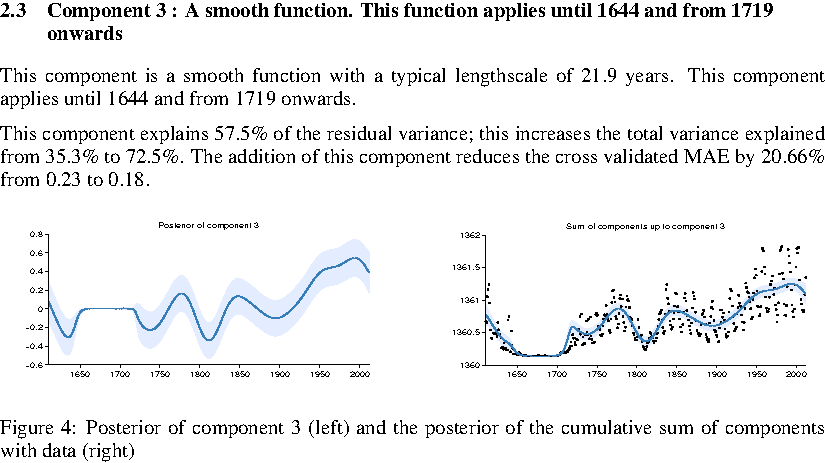
\includegraphics[width=0.98\columnwidth]{solarpages/02-solar-seperate-pages-6}}
%\caption{Characterizing the medium-term smoothness of solar activity levels.  By allowing other components to explain the periodicity, noise, and the Maunder minimum, we can isolate the part of the signal best explained by a slowly-varying trend.}
%\label{fig:smooth}
%\end{figure}

%\paragraph{Isolating the smoothly-varying component} Examining the dataset by eye, overall solar activity seems to change slowly over decades.  However, this intuition seems difficult to formalize.  Linear or quadratic regression is clearly inappropriate, and methods based on local smoothing would need to control for the periodic component.  Luckily, the GPSS procedure does exactly this, allowing us to isolate the slowly-varying component of the data, without having to forecast either the Maunder minimum or the periodic variation.  Figure \ref{fig:smooth} shows the automatically-generated summary of this component.

\begin{figure}[ht]
\centering
\fbox{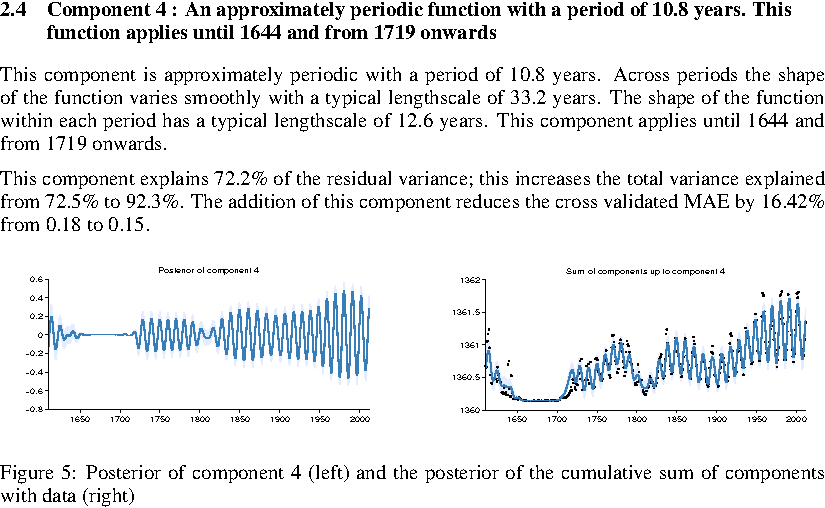
\includegraphics[trim=0cm 0cm 0cm 1.0cm, clip, width=0.98\columnwidth]{solarpages/02-solar-seperate-pages-7}}
\caption{Isolating the locally periodic component of the dataset.}
\label{fig:periodic}
\end{figure}

%Figure \ref{fig:periodic} shows that GPSS has identified the approximately 11 year solar cycle.
%By isolating this component in separate plots it is easy to see the exact nature of the solar cycle \eg how the amplitude of this periodic component varies over time.
%This demonstrates one benefit of isolating individual components: we can now see, by eye, extra structure that was not explicitly captured by the model.  Specifically, we can see that the amplitude of the periodic component varies over time.

%and by comparing with figure \ref{fig:smooth}, we can see that it varies roughly in proportion to the overall magnitude of the signal.
%  This pattern suggests that some sort of log-transform might be appropriate for this dataset, or that the model should be extended in some way to capture this structure.

%\paragraph{Extrapolation plots}
%
%The third section of each report shows extrapolations into the future, as well as posterior samples from each individual component of the model.  These samples help to characterize the uncertainty expressed by the model, and the extent to which different components contribute to predicting the future behavior of a time series.
%%
%The predictive mean and variance of the signals shown in the summary plots are useful, but do not capture the joint correlation structure in the posterior.  Showing posterior samples is a simple and universal way to illustrate joint statistical structure.
%%
%\begin{figure}[ht]
%\centering
%\fbox{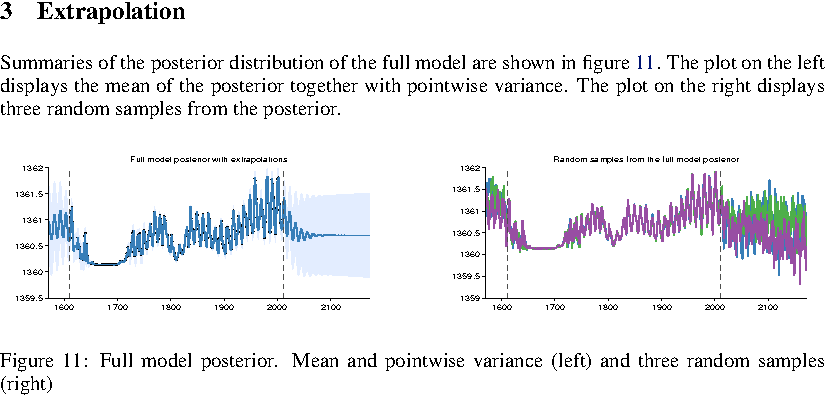
\includegraphics[trim=0cm 0cm 0cm 2.8cm, clip, width=0.98\columnwidth]{solarpages/02-solar-seperate-pages-13}}
%\caption{Sampling from the posterior.  These samples help show not just the predictive mean and variance, but also the predictive covariance structure.  Note, for example, that the predictive mean (left) does not exhibit periodicity, but the samples (right) do.}
%\label{fig:extrap-full}
%\end{figure}
%%
%For example,
%%  shows the predictive mean and variance given the entire model. 
%it is not clear from the left-hand plot in figure \ref{fig:extrap-full} whether or not the periodicity of the dataset is expected to continue into the future.  However, from the samples on the right-hand size, we can see that this is indeed the case.  

%\begin{figure}[h!]
%\centering
%\fbox{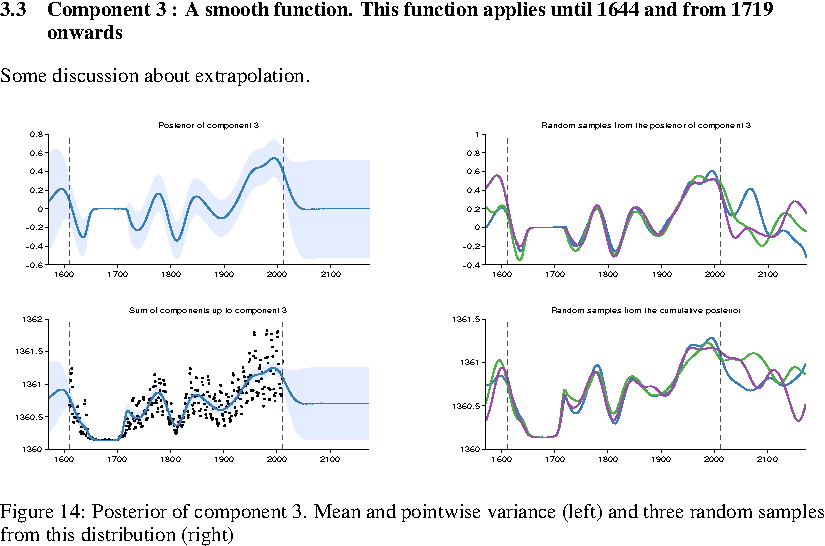
\includegraphics[width=0.98\columnwidth]{solarpages/02-solar-seperate-pages-16}}
%\caption{Extrapolating a single component of the model.  Because our model class allows us to isolate individual components, we can show the extent to which the model expects different trends to continue.  We also observe that the posterior samples are quite different from the posterior mean, away from the data.}
%\label{fig:extrap-smooth}
%\end{figure}

%\paragraph{Extrapolating individual components}
%We can also examine the model's expectations about the future behavior of individual components through sampling.  Further plots in the extrapolation section show posterior samples for each individual additive component. %For example, in figure \ref{fig:extrap-smooth}, we are shown samples of the predictive distribution of the smooth component of variation.  This plot indicates that the model considers a wide range of future average intensities to be plausible, but that it always expects those average intensities to vary smoothly.

%\section{Related Work}

%There exists a vast literature on both model visualization and model checking.


%\paragraph{Structure learning in Bayesian networks}
%Similar idea of discovering semantics via model search.
%Semantics are more vague though \ie a probability table is not an entirely concise summary

%\paragraph{Linear model}
%These discover highly interpretable semantics but are limited in expressivity

%\paragraph{Nonparametric additive models}
%Highly flexible but semantics are vague \ie can only talk about smooth functions

%\paragraph{Equation learning}
%Very flexible but semantics of equations do not map onto human understanding \eg saw tooth vs Fourier decomposition of a saw tooth - which is more human understandable?
%How would you explain a sensor error with Eureqa style equations.

%\paragraph{Deep learning}
%Again very flexible but the semantics are not usually human interpretable.
%How can we understand the output of complex representation learning algorithms without human intervention (\eg recognising that your deep net has become a cat classifier).

%\paragraph{Kernel search}
%Can use the precise semantics of linear models or the vague semantics of nonparametric additive models and other components along this spectrum.
%Flexible modelling with components that a human might use to describe what is going on.

\subsection{Describing heteroscedasticity}
\label{sec:airline}

\begin{figure}[h]
\centering
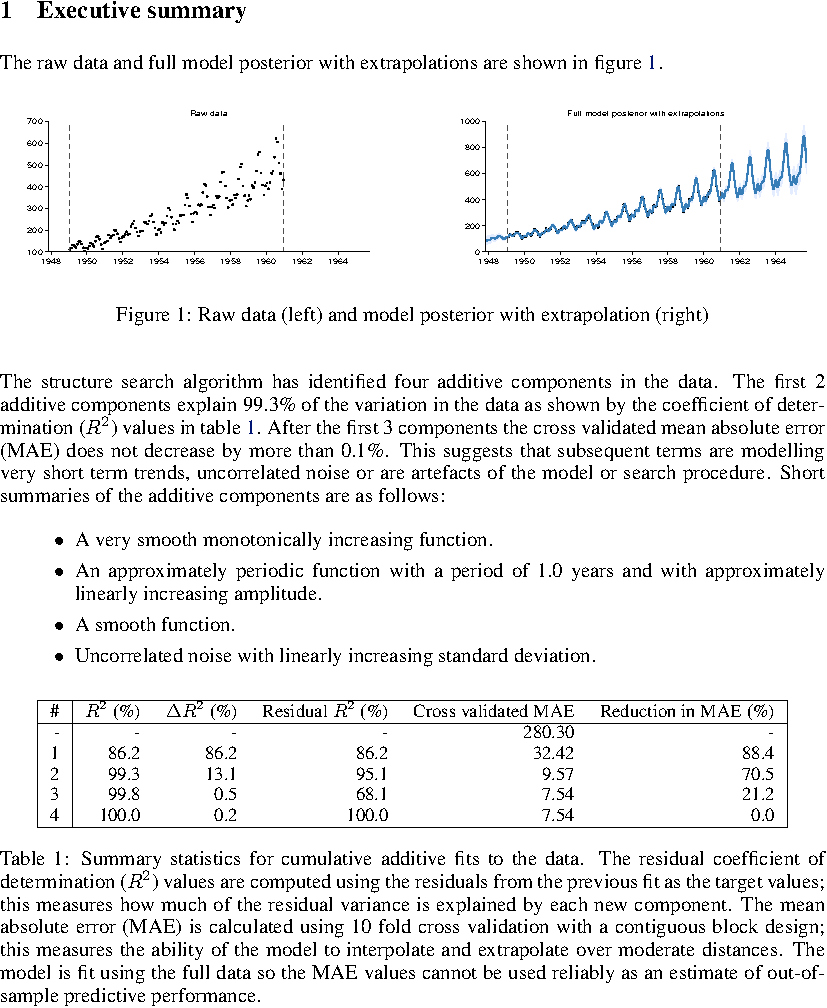
\includegraphics[trim=0cm 12.5cm 9cm 1.7cm, clip, width=0.98\columnwidth]{airlinepages/01-airline-separate-pages-2}
\caption{
International airline passenger data.}
\label{fig:airline}
\end{figure}

We also analysed international airline passenger data (figure~\ref{fig:airline}).
The model constructed by GPSS has four components with descriptions given in figure~\ref{fig:exec-airline}.
\vspace{-0.5\baselineskip}
\begin{itemize}
  \itemsep0em
  \item $\kSE$
  \item $\kSE \times \kPer \times \kLin$
  \item $\kSE$
  \item $\kWN \times \kLin$
\end{itemize}
\vspace{-\baselineskip}

\begin{figure}[h]
\centering
\fbox{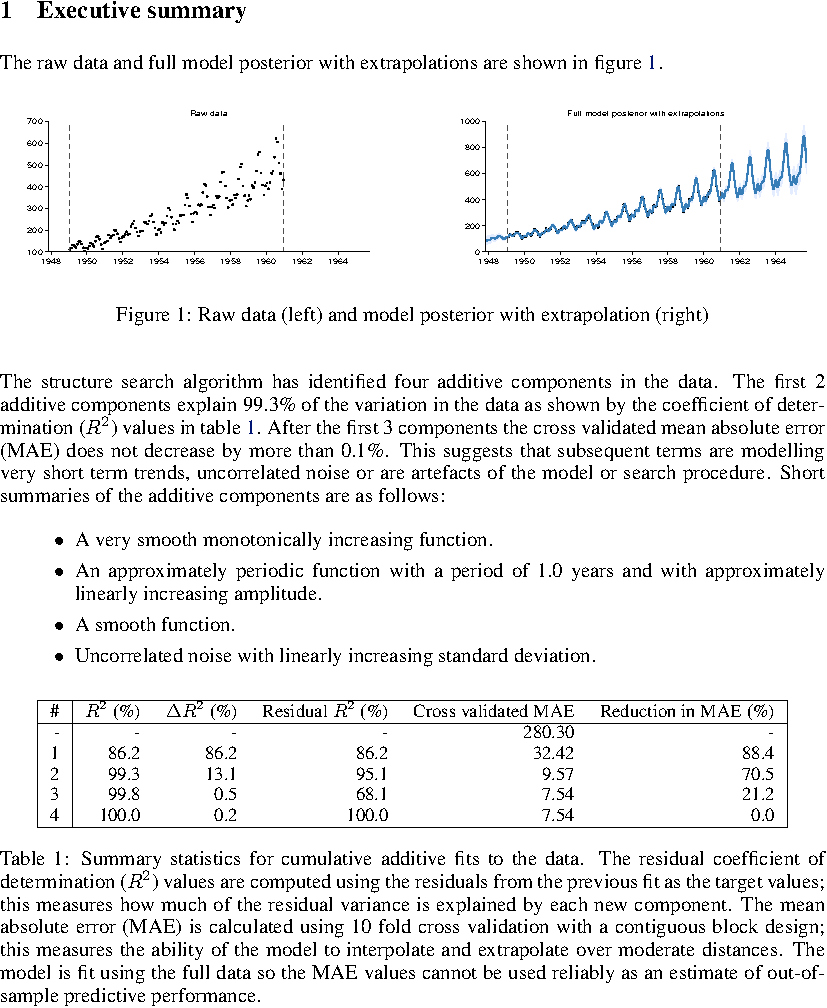
\includegraphics[trim=0cm 3cm 0cm 6cm, clip, width=0.98\columnwidth]{airlinepages/01-airline-separate-pages-2}}
\caption{
Short descriptions and summary statistics for the four components of the airline model.}
\label{fig:exec-airline}
\end{figure}

\paragraph{Monotonic trend}

No model in the current language can express a prior over monotonic functions.
However, it is simple to check the posterior for monotonicity and remark upon it when appropriate (figure~\ref{fig:monotonic}).

\begin{figure}[h]
\centering
\fbox{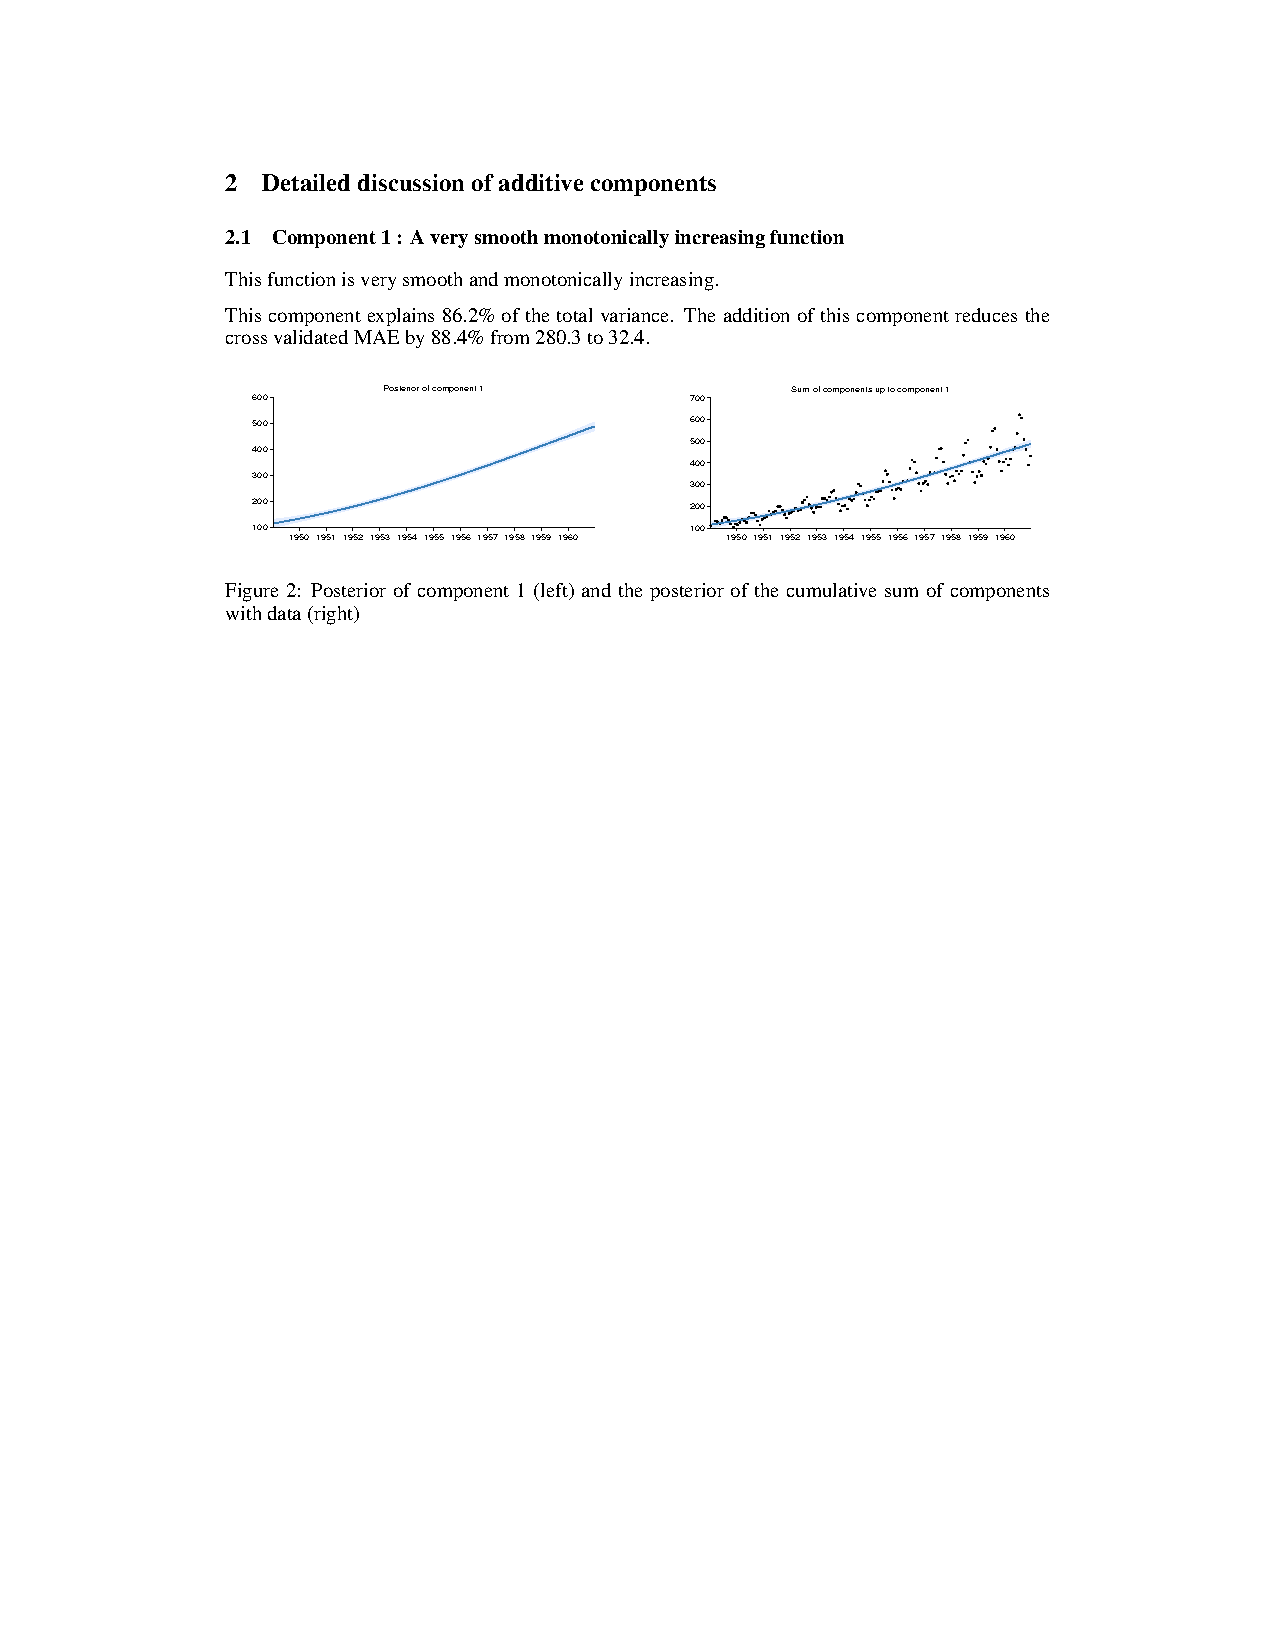
\includegraphics[trim=0cm 0cm 0cm 0cm, clip, width=0.98\columnwidth]{airlinepages/01-airline-separate-pages-3}}
\caption{Describing monotonicity of the posterior}
\label{fig:monotonic}
\end{figure}

\paragraph{Annual periodicity with linearly growing amplitude}

The second component (figure~\ref{fig:lin_periodic}) is correctly identified as approximately ($\kSE$) periodic ($\kPer$) with linearly growing amplitude ($\kLin$).

\begin{figure}[h]
\centering
\fbox{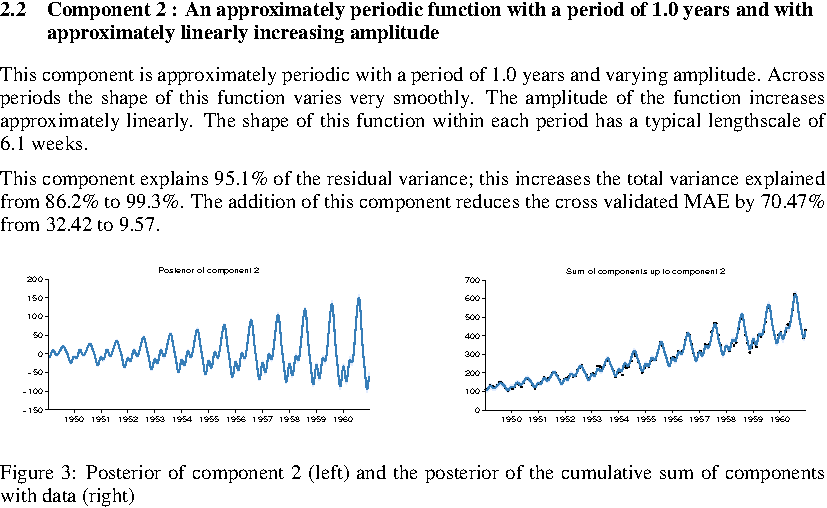
\includegraphics[trim=0cm 0cm 0cm 0cm, clip, width=0.98\columnwidth]{airlinepages/01-airline-separate-pages-4}}
\caption{Capturing non-stationary periodicity in the airline data}
\label{fig:lin_periodic}
\end{figure}

%\begin{figure}[h]
%\centering
%\fbox{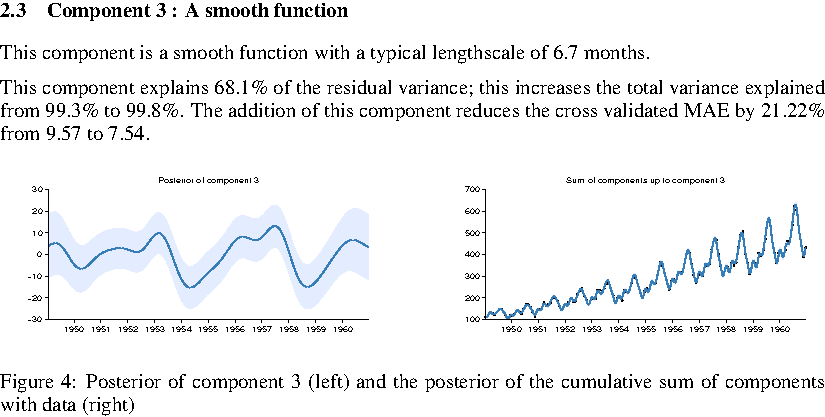
\includegraphics[trim=0cm 17cm 0cm 3.5cm, clip, width=0.98\columnwidth]{airlinepages/01-airline-separate-pages-5}}
%\caption{
%A caption.}
%\label{fig:exec}
%\end{figure}

\paragraph{Linear heteroscedasticity}

By multiplying a white noise kernel by a linear kernel the model is able to express heteroscedasticity (figure~\ref{fig:heteroscedastic}).

\begin{figure}[h]
\centering
\fbox{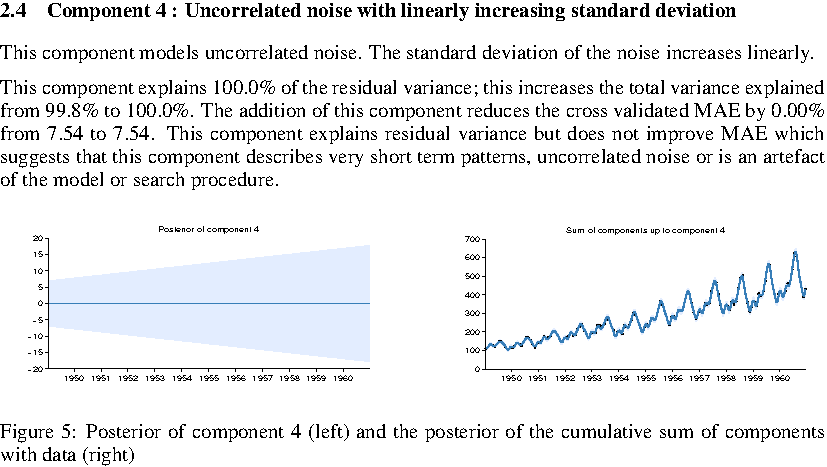
\includegraphics[trim=0cm 0cm 0cm 0cm, clip, width=0.98\columnwidth]{airlinepages/01-airline-separate-pages-6}}
\caption{Modelling heteroscedasticity}
\label{fig:heteroscedastic}
\end{figure}

\subsection{Comparison to equation learning}

Much of machine learning research focuses on numerical performance, with claims of interpretability generated post-hoc.
In contrast, equation learning \citep{Schmidt2009b} can also be used to automate the process of interpretation.

We include learned equations for these two data sets produced using Eureqa \citep{Eureqa} using the default mean absolute error performance metric\footnotemark.
\footnotetext{We experimented with the root mean squared error with Akaike information criterion penalisation (this is most comparable to the Bayesian information criterion used by GPSS) but occasionally observed severe overfitting.}
However, it is very unlikely that these data sets can be explained parsimoniously with a parametric function.

The learned equation for the solar irradiance data is
\begin{equation}
\textrm{Irradiance} = 1361 + \alpha\sin(\beta + \gamma t)\sin(\delta + \epsilon t^2 - \zeta t)
\end{equation}
where $t$ is time (the input to the regression) and we have replaced most constants with symbols for brevity.
This equation captures the constant offset of the data and models the long term trends with a product of sinusoids but fails to capture the solar cycle or the Maunder-minimum.

The learned equation for the airline passenger data is
\begin{equation}
\textrm{Passengers} = \alpha t + \beta\cos(\gamma - \delta t)\textrm{logistic}(\epsilon t - \zeta) - \eta
\end{equation}
which captures the approximately linear trend, and the periodic component with approximately linearly (logistic) increasing amplitude.
However, the periodicity is heavily approximated with only a single sinusoid and the model cannot capture heteroskedasticity.

\section{Related work}

\paragraph{Building Structured Covariance Functions}

\cite{rasmussen38gaussian} devotes 4 pages to constructing a complex kernel to model the time series of Mauna Loa carbon dioxode conentrations over time.  An automatic report showing similar structure is contained in the supplementary material.  Other examples of papers whose main contribution is constructing and fitting a compound gp{} kernel are \cite{klenske2012nonparametric} and \cite{lloydgefcom2012}.

Contrast with kernels preserving group symmetries???

\paragraph{Equation learning}

%In this work we have defined a search space of statistical models, where each model is characterised by a parametric covariance function.
%Previous work has considered searching over parametric functions \citep[e.g.][]{Schmidt2009b}.
%Some functions are well explained parametrically \eg a logistic function, whereas others are best described by their covariance \eg an approximately periodic function.
\cite{schmidt2009distilling}, \cite{todorovski1997declarative} and \cite{washio1999discovering} learn parametric forms of equations specifying time series, or relations between quantities.  Because our system specifies the more general covariance structure rather than the functions themselves, we are able to capture structure which does not have a simple parametric form.

\paragraph{Searching over statistical models}

GPSS was originally inspired by the search over matrix factorisation models by \cite{grosse2012exploiting}.
Automatic model search is possible whenever the following conditions are met: 1) we can define a large space of models by combining a small number of components in a small number of different ways, inference can be performed for all models in this space, and a basic search procedure is sufficient to find accurate models.  For example, \citet{kemp2008discovery} learned the structural form of a graph used to model human similarity judgments.  

More generally, probabilistic programming [cite] software automatically generates inference mechanisms for open-ended classes of models, enabling automatic model search.  For example, \cite{VikashScene13} automatically searches over models of 2D scenes.

%\NA{
%This is also true of - can we also cite some sort of graphical model work?
%}
%\fTBD{RG: Cite Kemp + Tenenbaum?}

%\paragraph{Standard inference methods}
%\fTBD{RG: How is this relevant?}
%The GPSS language can express many regression motifs as \gp{}s for which inference is well understood.
%Probabilistic programming (cite) defines languages that describe generative models in such a way that %inference can be performed in each model.
%Extending the model search ideas in GPSS to searches over probabilistic programs would be an interesting area for future research (cite Josh's workshop paper?).

\paragraph{Natural-language descriptions of data}

To the best of our knowledge, our procedure is the first example of automatic description of nonparametric statistical models.% is novel (whereas parametric models are typically described by their parameters).
However, grammar based techniques have previously been used to automatically understand images \cite{zhu2007stochastic} and recently \citet{GanesalingamG13} produced a theorem proving system that expresses its proofs in natural language.








\section{Numerical evaluation}
\label{sec:numerical}

To complement our demonstration of the interpretability of our method, we conducted numerical experiments testing the ability of various model building algorithms to interpolate and extrapolate time-series.
GPSS outperforms the other methods on average (\eg as measured by quantiles of performance metrics).
\NA{However, the variability of the results suggests that there is room to improve the robustness of GPSS.}
\fTBD{I'm trying to avoid claims of oversell - any thoughts on a measured statement?}

\subsection{Data sets}

In addition to the three time series analysed in \cite{DuvLloGroetal13} we evaluate the performance of GPSS and 5 other algorithms on 10 additional time series from the time series data library \citep{TSDL}; plots can be found at the beginning of the reports in the supplementary material.

\subsection{Algorithms}

We compare the structure search algorithm to equation learning (EL) using Eureqa \citep{Eureqa} and four other regression algorithms; additive nonparametric regression (SE) \citep[e.g.][]{buja1989linear}\fTBD{This reference is not quite correct}, change point modelling (CP) / multi resolution Gaussian processes \citep[e.g.][]{garnett2010sequential, FoxDunson:NIPS2012}, spectral kernels (SP) \citep{WilAda13} and trend-cyclical-irregular (TCI) \citep[e.g.][]{lind2006basic}\fTBD{Can anyone find a more academic reference?}.

We use the default mean absolute error criterion when using Eureqa.
The other four algorithms can be expressed as restrictions of our modelling language (see table~\ref{table:motifs}) so we perform inference using the same search methodology and selection criterion\footnotemark~(Bayesian information criterion) with appropriate restrictions to the grammar.
For SE, SP and TCI this corresponds to a forward selection algorithm.
\footnotetext{We experimented with using unpenalised conditional likelihood as the search criterion for other methods but observed overfitting as is to be expected.} 

We restricted to regression algorithms for comparability; this excludes models which regress on previous values of times series \citep[e.g.][]{box2013time}.
Producing model construction algorithms for this class of time-series model would be an interesting area for future research.

\subsection{Inference}

We use exact inference, as in \cite{DuvLloGroetal13}.
\fTBD{JL: This is way to short - search operators?}

\subsection{Interpretability versus accuracy}

Since the process of describing a model always converts a kernel into a sum of products we experimented with always keeping the kernel in this form.
After applying search operators to a kernel we distributed all products over addition, changepoint and changewindow operators and simplified the resulting expression.
This variant (GPSS.SoP) of the search tends to produce models with fewer additive components improving interpretability but does not perform as well numerically.

The research leading up to this manuscript has focused on interpretability.
One could almost certainly improve the numerical results presented in this section by reintroducing $\kRQ$ and including Mat\'ern kernels as well as others.
We leave a full exploration of the interpretability / accuracy trade-off for future work.

\subsection{Extrapolation}

To test extrapolation we trained all algorithms on the first 90\% of the data, and attempted to predict the remaining 10\% and then computed the root mean squared error (RMSE).
The values of the RMSEs are then standardised by dividing by the smallest RMSE for each data set \ie the best performance on each data set will have a value of 1.

Figure~\ref{fig:box_extrap_dist} shows the standardised RMSEs across algorithms.
Both versions of GPSS have lower quartiles than all other methods but the outliers of GPSS, TCI and SP have similar values.

\begin{figure}[h]
\centering
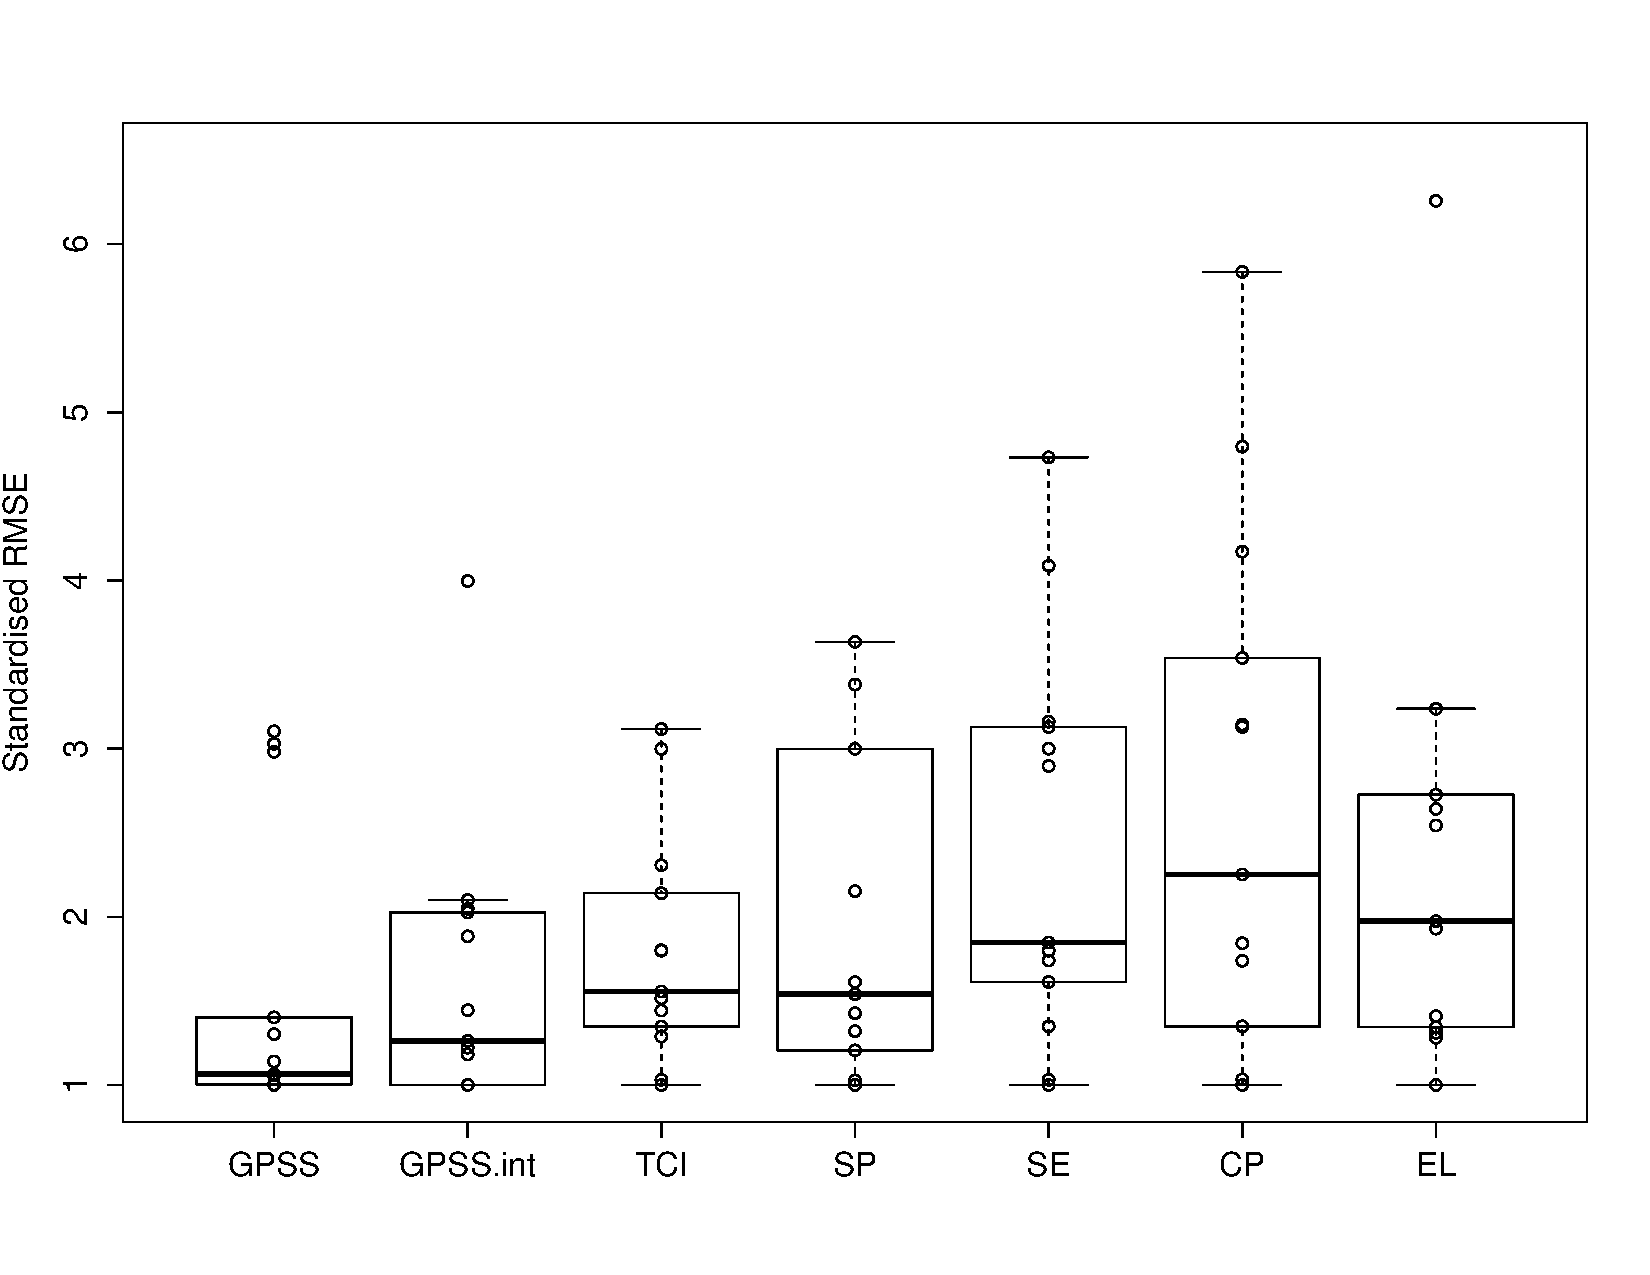
\includegraphics[width=\columnwidth]{figures/box_extrap_dist}
\caption{
Raw data, and box plot of standardised extrapolation RMSE (best performance = 1).
Ordered by median.
}
\label{fig:box_extrap_dist}
\end{figure}

Not shown on the plot is a large outlier for SP of 11 on a dataset with a large and sharp discontinuity (see the call centre data in the supplementary material) which violates its assumptions of stationarity.

Also not shown on the plot is a very large outlier for EL of 493 (this was also on the call centre data).
However, EL was the best performing algorithm on the wages dataset which shows an exponential increase after the industrial revolution.
GPSS can approximate an exponential function with a polynomial by combining $\kLin$ kernels but this is not a succinct expression in the current language.
Expanding the modelling language of GPSS is a natural area for future research.

Somewhat surprisingly, TCI performs well despite its restrictive modelling assumptions (smooth functions and exact periodicity).
Further inspection of the extrapolation has revealed that while TCI cannot model non-stationarity, its extrapolations of approximately periodic components can be quite effective.
While GPSS and SP will quickly become uncertain about a roughly periodic component, TCI will predict the average which is often more effective.
This suggests that models composed of kernels of the form $(\kSE + \kC) \times \kPer$ will be effective for extrapolating approximately periodic components.

\subsection{Interpolation}

To test the ability of the methods to interpolate, we randomly divided each data set into equal amounts of training data and testing data.
We trained each algorithm on the training half of the data, produced predictions for the remaining half and then computed standardised RMSEs.

The results are similar to those for extrapolation and are deferred to the supplementary material for brevity.

\section{Discussion}

\TBD{Help requested - haven't thought of a definitive conclusion myself}

Towards the goal of automating the process of statistical analysis we have introduced a system that can automatically describe the complex statistical models it produces.

In the earlier work of \cite{DuvLloGroetal13} the GPSS procedure was applied to multidimensional inputs; we see no obstacles to extending the work in this manuscript to multidimensional inputs.

\paragraph{Disconnected unordered notes}

Changepoints and heteroscedasticity now included leading to increased expressivity and interpretability.

GPSS superior at extrapolation and interpolation, but results are high variance - robustness needs to be improved (which probably means a better search algorithm).

Automatically generating descriptions makes interpretability objective - rather than a post-hoc step performed by experts.

Describing complex statistical models makes them more transparent to the non-expert user.

If we can explain something in plain language then we should.

The improved grammar is a machine learning contribution - the description is an AI contribution (there was no learning involved, just the application of rules).

We encourage others to make their models automatically describable - but what are the metrics of success at this task?
For statistical regression the ultimate measure of success is a scientific discovery based on an automated analysis - but we are a way off from that (need to go into higher dimensions with better search I think).

\paragraph{Source Code}
Source code to perform all experiments is available on github.\footnote{Available upon publication}
%\href{http://www.github.com/jamesrobertlloyd/gpss-research}
%{\texttt{github.com/jamesrobertlloyd/gpss-research}}}
%All \gp{} hyperparameter tuning was performed by automated calls to the GPML toolbox\footnote{Available at 
%\href{http://www.gaussianprocess.org/gpml/code/}
%{\texttt{www.gaussianprocess.org/gpml/code/}}
%}

%\section{Discussion}

%\begin{quotation}
%``The availability of 'user-friendly' statistical software has caused authors to become increasingly careless about the logic of interpreting their results, and to rely uncritically on computer output, often using the 'default option' when something a little different (usually, but not always, a little more complicated) is correct, or at least more appropriate.''
% In trying to practice this art, the Bayesian has the advantage because his formal apparatus already developed gives him a clearer picture of what to expect, and therefore a sharper perception for recognizing the unexpected.

%\defcitealias{dyke1997avoid}{G. Dyke, 1997}
%\hspace*{\fill}\citet{Jaynes85highlyinformative}
%\hspace*{\fill}\citetalias{dyke1997avoid}
%\end{quotation}

%In this paper, we exhibited the output of a method for automatically constructing and summarizing a compositional Gaussian process regression model in natural language.
%These summaries can enable human experts and non-experts to understand the implications of a model, check its plausibility, and notice structure not yet captured by the model.

\bibliography{gpss}
\bibliographystyle{format/icml2014}

\end{document} 
